\begin{abstract}
A frozen next-scale image model can complete a representation from a transmitted prefix, but whole-scale stopping points need not use a finite digital frame efficiently. NeST-Com admits raster-ordered endpoints inside a scale, conditionally entropy-codes the selected tokens, and falls back through a frozen chain until the actual terminated stream fits. A paid profile identifies the endpoint and channel layout; an isolated receiver entropy-decodes transmitted tokens before generating the unsent part. At 1024 complex channel uses, the corrected 19-dB comparison on 500 images improves PSNR by 0.319 dB over the same-prior entropy-coded whole-scale family, with a 95\% source-paired interval of [0.290, 0.349] dB. Low-SNR pixel fidelity and perceptual metrics still favor different baseline systems. A separate matched 100-source study adapts native ARPC to the same digital budget. At 2048 uses, finite calibration selects equally protected two-fragment policies for 4/10 dB. All 1200 test objects across the two methods are correctly received, and NeST-Com's paired PSNR gains are 3.779 and 3.877 dB; all seven metrics favor it at these two points. A distinct 19-dB test delivers both complete representations: ARPC then has lower DISTS, while DINO and prediction-agreement intervals cross zero. The results identify useful finite-budget operating points and their boundaries without attributing all system differences to endpoint granularity.
\end{abstract}
\begin{IEEEkeywords}
Digital image transmission, conditional entropy coding, visual autoregressive model, finite frame budget, link adaptation.
\end{IEEEkeywords}

\section{Introduction}
\IEEEPARstart{G}{enerative} image models enable a receiver to infer information omitted by a transmitter. Their usefulness over a digital link depends on the information that actually survives the source parser and channel decoder. A compact representation does not by itself specify a feasible frame: termination, syntax, profile signaling, error detection and channel protection must all fit the available channel uses.

Next-scale visual autoregressive (VAR) models predict residual token maps from coarse to fine~\cite{tian2024var}. They naturally support reconstruction from complete coarse scales. However, the available channel-code capacities are not generally aligned with those scale boundaries. For example, seven and eight VAR scales contain 155 and 255 tokens. A frame able to carry more than the former but less than the latter cannot use the intermediate source capacity if only whole-scale endpoints are admitted. Conditional entropy coding changes the actual number of bits, but does not eliminate the discreteness of the allowed endpoints.

We study the transmission interface under a \emph{hard per-image digital frame budget}. The main implementation of \nest{} conditionally entropy-codes a legal within-scale prefix. Its target endpoint and modulation/coding scheme (MCS) are selected offline from finite candidates. At transmission time, only the observed terminated source length controls fallback along a frozen chain. The paid profile specifies the actual endpoint and layout. At reception, the shared model reconstructs entropy probabilities from already decoded tokens, then completes only the unsent part. A raw-index variant avoids transmitter-side probability inference and is retained as an auxiliary implementation.

The contribution is this finite-budget interface and its evaluated tradeoffs: legal within-scale endpoints, explicit terminated-length accounting, paid endpoint signaling and an isolated receiver. The tokenizer, generative prior, arithmetic coding principle and pretrained perceptual metrics are inherited components. Offline calibration is finite candidate selection, not a new search algorithm. Internal whole/partial comparisons test the value of the extra endpoint choices; an external ARPC comparison tests the complete adapted systems and cannot isolate endpoint granularity by itself.

\section{Related Work and Scope}
Deep JSCC learns continuous mappings from images to channel symbols and avoids a separate hard source parser~\cite{bourtsoulatze2019deep}. SwinJSCC uses Transformer representations and channel adaptation~\cite{yang2023swinjscc}. Such methods provide an important contrast to finite-block digital transmission: their graceful degradation can be favorable for low-SNR pixel fidelity, while their learned representations, losses and auxiliary signaling differ from the present scheme.

Generative reception adds a prior to the information carried by the observation. DiffCom uses the channel observation in diffusion posterior sampling~\cite{wang2025diffcom}. Token communication offers another interface between learned representations and a digital link~\cite{qiao2025tokcom}. VAR supplies the frozen next-scale prediction mechanism used here~\cite{tian2024var}. ARPC combines progressive autoregressive coding with native source syntax and generation~\cite{arpc2026}; our external experiment preserves its native source representation and charges its caption and mode information before LDPC--QAM transmission. Ada-TokenCom integrates autoregressive token compression and generation with dynamic source/MCS control~\cite{adatokencom2026}. In contrast, our study fixes each frame's channel-use budget and evaluates a finite, frozen endpoint/MCS policy with actual source-length fallback.

These relationships narrow the novelty claim. We do not introduce next-scale prediction, entropy coding, text-conditioned image generation or a generic principle of transmitting a prefix and generating its suffix. The question is whether a finer, fully charged source interface gives useful operating points between existing whole-scale boundaries, and where its advantage ends when a larger budget admits complete representations.

\section{Fixed-Budget Entropy-Coded Transmission}
\begin{figure*}[t]
\centering
\begin{tikzpicture}[font=\sffamily\scriptsize,box/.style={draw=black!65,fill=white,minimum height=13mm,align=center,inner sep=2pt},arr/.style={-{Latex[length=1.4mm]},thick}]
\node[box,text width=15mm] (tok) at (0,0) {VAR\\tokenizer};
\node[box,text width=30mm,right=4mm of tok] (src) {Conditional source coding\\terminated-length fallback};
\node[box,text width=23mm,right=4mm of src] (frame) {Paid profile\\CRC / LDPC / QAM};
\node[box,text width=11mm,right=4mm of frame] (ch) {AWGN};
\node[box,text width=25mm,right=4mm of ch] (parse) {Actual decode\\source parser};
\node[box,text width=23mm,right=4mm of parse] (gen) {Received tokens\\VAR completion};
\node[box,text width=12mm,right=4mm of gen] (dc) {$D_c$\\image};
\foreach \a/\b in {tok/src,src/frame,frame/ch,ch/parse,parse/gen,gen/dc}{\draw[arr] (\a.east)--(\b.west);}
\node[above=3mm of src,font=\sffamily\small] {Transmitter};
\node[above=3mm of gen,font=\sffamily\small] {Receiver};
\node[below=3mm of parse,align=center,text width=48mm] (gray) {Header / CRC / syntax rejected $\rightarrow$ fixed gray};
\draw[arr] (parse.south)--(gray.north);
\end{tikzpicture}

\caption{Main entropy-coded path. The actual terminated stream length selects a legal endpoint in a frozen fallback chain. The paid profile identifies that endpoint and the body layout. Entropy decoding recovers transmitted tokens; subsequent VAR completion generates unsent tokens. Invalid headers, CRCs or source syntax produce the fixed gray output. Raw serialization is an alternative interface, not a second simultaneous payload.}
\label{fig:system}
\end{figure*}

\subsection{Representation and Legal Endpoints}
A frozen tokenizer maps a $256\times256$ RGB image $\mathbf x$ to ten residual token maps $\mathbf r_1,\ldots,\mathbf r_{10}$. Their side lengths are $(1,2,3,4,5,6,8,10,13,16)$, and each token indexes a 4096-entry codebook. Let $L_s$ be the number of positions at scale $s$. All scales contain 680 tokens and accumulate into a $32\times16\times16$ residual latent decoded by $D_c$.

An endpoint $e=(m,K)$ transmits
\begin{equation}
 \pi_e(\mathbf x)=[\operatorname{vec}(\mathbf r_1),\ldots,\operatorname{vec}(\mathbf r_m),\mathbf r_{m+1}[1{:}K]],
\label{eq:endpoint}
\end{equation}
where positions follow the registered raster order. For $m<10$, $0\leq K<L_{m+1}$; a fully transmitted boundary scale is canonically $(m+1,0)$. Endpoint $(10,0)$ transmits the complete representation. The entropy-coded families use whole endpoints and, in the partial family, prescribed quarter-scale endpoints. The corrected candidate universe includes complete $m=10$ symmetrically in both families. The trained visual models and sampling rule are not changed when an endpoint is added.

\subsection{Conditional Coding and Actual-Length Fallback}
The null-class VAR produces integer cumulative distributions of total mass $2^{24}$ for a 32-bit arithmetic coder. Coarse scales are coded in order. The first $K$ positions of the boundary scale use their conditional distributions given the complete coarser maps. Let $b(\mathbf x,e)$ denote the \emph{actual terminated} stream length, including the coder's finish operation. A length estimate or an un-terminated entropy sum is not used for admission.

A policy $a$ specifies an MCS, a target endpoint and an ordered fallback chain $\mathcal F_a$. Its LDPC information length is $k_a$. The selected endpoint is the first legal member of the frozen order satisfying
\begin{equation}
 b(\mathbf x,e)+13+16\leq k_a.
\label{eq:fit}
\end{equation}
The 13-bit length and 16-bit body CRC are paid separately. Known padding fills the information block. No reconstruction is generated at the transmitter to choose among fallback endpoints, and no test metric enters this decision. If the chain has no fitting member, a null profile is transmitted and that source remains in the failure denominator. This source-side capacity fallback is distinct from the receiver's output after a channel failure.

The 12-bit public profile ID is protected by CRC16, six convolutional tail bits and rate matching to 136 coded bits. It occupies 68 QPSK symbols. The recovered profile identifies the actual $(m,K)$, source syntax and body-code layout. The stream length field delimits the arithmetic payload; it does \emph{not} independently determine how many tokens or which endpoint were transmitted.

\subsection{Channel and Resource Accounting}
At the primary budget $N=1024$, the entropy body occupies 956 symbols. For $q=\log_2M\in\{2,4,6\}$,
\begin{equation}
 n_a=956q,\qquad 68+\frac{n_a}{q}=1024.
\end{equation}
The backend uses a supported 5G NR LDPC block with its actual lifting, information length and rate matching~\cite{3gpp38212}. Nominal rates label candidates; feasibility uses the actual integer $k_a,n_a$. For example, the corrected 19-dB layout has $k_a/n_a=4780/5736$, leaving 4751 source bits after the two fields in (\ref{eq:fit}).

For every method, constellations have nominal average symbol energy $E_s=2$. With $\mathbf y=\mathbf s+\mathbf n$ and $\mathbf n\sim\mathcal{CN}(\mathbf0,N_0\mathbf I)$,
\begin{equation}
 N_0=2\,10^{-\mathrm{SNR}_{\mathrm{dB}}/10}.
\end{equation}
The digital QAM frame's realized energy depends on its symbol composition; it is recorded rather than normalized per frame. Comparisons use the declared nominal energy convention. There is no feedback, retransmission or power allocation. The normalized primary budget is $N/(3\cdot256^2)=1/192$ complex channel uses per source component.

\subsection{Receiver Isolation and Completion}
The receiver sees the actual received symbols, public profiles and shared frozen models. It first decodes the protected header, then the LDPC body. Header rejection, CRC failure, invalid length or padding, and arithmetic syntax/termination failure produce the fixed RGB-0.5 image. The entropy implementation never retains a damaged arithmetic stream or assumes that a correct coarse prefix survives its failed CRC.

For an accepted source object, the receiver constructs the same integer CDFs from the already decoded coarse tokens. It receives no transmitter CDF, source pixel, hidden embedding, untransmitted token or oracle error correction. Once the transmitted tokens are recovered, complete maps condition the next-scale prior. At a partially transmitted map, the model predicts the map, the received positions overwrite their predictions, and the merged map advances the latent state:
\begin{equation}
 \widetilde r_{m+1,j}=\begin{cases}
 \widehat r_{m+1,j},&j\leq K,\\
 \arg\max_v p_{\mathrm{VAR}}(v\mid\widehat{\mathbf r}_{\leq m}),&j>K.
 \end{cases}
\end{equation}
Finer unsent maps are generated from that state and $D_c$ reconstructs the image. Source/CDF equality is audited only after output is fixed; audit truth cannot change the receiver result. Independent-process round trips check this boundary with actual source streams.

\subsection{Frozen Models, Calibration and Raw Variant}
The tokenizer and VAR remain pretrained and frozen. Before link evaluation, $D_c$ was adapted on the same 20,000 training images using MSE$+0.1$LPIPS and a mixture of continuous, fully quantized and completed-prefix latents. Its checkpoint was selected on the 1000-source calibration set, then frozen and shared with latent-space JSCC. This earlier adaptation is disclosed; the present evaluation trains no model.

For a finite candidate set $\mathcal A_\gamma$, each complete policy includes its target and fallback chain. Selection uses actual received-image DINOv2-L cosine similarity $Q$~\cite{oquab2024dinov2}:
\begin{equation}
 \widehat a_\gamma=\arg\max_{a\in\mathcal A_\gamma}
 \frac{1}{|\mathcal C|}\sum_{i\in\mathcal C}\frac{1}{3}\sum_{\ell=1}^{3}Q(\mathbf x_i,\widehat{\mathbf x}_{i,a,\ell}).
\label{eq:select}
\end{equation}
Failures remain included and the registered deterministic tie rule is retained. Clean-quality/link-probability screening only nominates candidates; it is not a measured wireless result. Test images cannot change policies, checkpoints or metric definitions.

The auxiliary raw interface serializes each selected token in 12 bits and avoids transmitter VAR probability inference. Its historical registered receiver retains actual LDPC hard decisions after body-CRC rejection (KEEP), while header failure remains gray. Thus raw and entropy implementations differ in source coding \emph{and} framing/failure rules. Cross-interface comparisons are system comparisons, not a pure two-factor causal ablation. The entropy receiver never inherits raw KEEP.

\section{Evaluation Protocol and Version Control}
\subsection{Populations, Metrics and Baselines}
The original split contains 20,000 training images, 1000 calibration sources, 100 development sources and 500 evaluation sources (common500). A separate independent new100 is reported separately. The external comparison uses the registered external\_common100\_v1 subset of common500; it is a matched subset, not a new blind population. Calibration-only cal100 clean diagnostics and the fixed16 development gallery have separate roles and denominators.

The primary entropy evaluation uses 4, 10 and 19 dB, with three noise draws per source. Metrics are PSNR, LPIPS-Alex~\cite{zhang2018lpips}, DINOv2-L cosine similarity, ConvNeXt-Tiny top-1 prediction agreement~\cite{liu2022convnext}, DISTS~\cite{ding2021dists}, DreamSim~\cite{fu2023dreamsim} and MS-SSIM~\cite{wang2003msssim}. Agreement is the fraction whose reconstruction prediction matches the source-image prediction. Neither agreement nor feature cosine is a semantic-correctness percentage. Official metric implementations, weights, normalization and preprocessing are frozen; DreamSim uses its registered ensemble and 224-square bicubic antialiased preprocessing. All directions are reported, including conflicting metrics.

\emph{Latent-space JSCC} communicates the continuous latent using convolutional communication layers and the same $D_c$. Its final 100k checkpoint was trained with MSE, LPIPS and a latent loss on the common training set. Its $2N$ real channel outputs form $N$ complex symbols with total energy $2N$. \emph{SwinJSCC (adapted)} uses the author's SA+RA architecture~\cite{yang2023swinjscc}, the same training set and the final 200k checkpoint. At $N=1024$, its six-channel representation occupies 768 symbols; the other 256 carry protected auxiliary mask/power information obtained at the receiver from the actual header. \emph{Adaptive BPG + LDPC}~\cite{bellard2014bpg} uses a frozen resolution/quantization procedure and a calibration-selected MCS, charging the complete source file and digital overhead. These are final checkpoints and registered adapters, not claims of equal architectures, losses or training convergence.

\subsection{Statistics and Evidence Identity}
We first average the three channel realizations within each source. Means and direct paired differences use the existing 10,000-replicate source bootstrap from each registered study. Whole/partial intervals are formed from source-paired differences, never by subtracting two marginal intervals. Intervals are pointwise and not multiplicity-adjusted; they do not cover training randomness or all model-design choices. A cross-zero interval does not establish equivalence. When historical methods use different channel seeds, matching is by source, not an assertion of identical channel observations.

At 19 dB, both entropy-coded families use the T1-C m10 correction. All 600 source traversals preserve the earlier 24 endpoints byte-for-byte in the frozen implementation. Complete m10 fits only 6/500 common500 and 1/100 new100 sources at 4751 bits; the rest follow their frozen family-specific chains. The older common500 whole-scale streams were produced in a different implementation environment and are not silently inherited. T1-C verifies complete event identities and updates changed events; its old-to-new difference combines version and m10 effects and is not a pure m10 ablation. The 4/10-dB results retain their frozen policies, subject to the explicit consistency audit below.

\subsection{Same-Version Source Utilization Audit}
The accompanying audit is restricted to common500, two entropy families and three SNRs: 3000 source records. Source statistics count one terminated stream per source/family/SNR, not three copies for three channel realizations. Utilization is $b(\mathbf x,e)/(k_a-13-16)$, with the actual endpoint, source capacity, spare capacity, stream version and source identity recorded together. Endpoint equality alone cannot establish reuse: the transmitted stream, paid header, actual receive event, reconstruction and score identity must also agree.

\begin{table}[t]
\centering
\caption{Same-version common500 source utilization, including arithmetic termination. Each cell is whole / partial. Capacity excludes the paid 13-bit length and CRC16; source statistics count each image once. These are source-layout statistics, separate from repaired wireless quality.}
\label{tab:utilization}
\footnotesize\setlength{\tabcolsep}{4pt}
\begin{tabular}{lrrr}
\toprule
SNR (dB) & Capacity (bit) & Utilization (\%) & Spare (bit) \\
\midrule
4 & 1245 & 73.81 / 93.08 & 326.0 / 86.1 \\
10 & 2520 & 77.70 / 95.21 & 561.9 / 120.8 \\
19 & 4751 & 85.24 / 94.73 & 701.2 / 250.3 \\
\bottomrule
\end{tabular}
\end{table}

Table~\ref{tab:utilization} reports the completed source-layout audit. Partial endpoints raise mean utilization from 73.81\% to 93.08\% at 4 dB, from 77.70\% to 95.21\% at 10 dB, and from 85.24\% to 94.73\% at 19 dB. The 500-source distributions use actual terminated lengths, not lengths inferred from token counts or a distribution reconstructed from means. Higher utilization alone is not a wireless quality gain; the version-consistent receive outputs are required for that conclusion.

The completed identity audit and minimal repair cover all 9000 logical frames. All 3000 partial-family frames at 4/10 dB and all 3000 T1-C frames at 19 dB are reused. Historical whole-family streams at 4/10 dB do not all match the current source version: exact matches reuse 9 and 570 frames, respectively, and the remaining 1491 and 930 are repaired under the original frozen policies. Thus 6579 logical frames are reused and 2421 physical events are newly evaluated, with 4842 header/body decoder calls. There is no new tokenizer or transmitter-probability traversal. The 807 distinct missing actual receiver outputs and their seven metrics are completed; unchanged source-paired bootstrap indices are reused with no new draws. These closed outputs, rather than the superseded historical whole-family scores, now support the quality comparison below.


\section{Results at the Primary Budget}
\begin{figure*}[t]
\centering
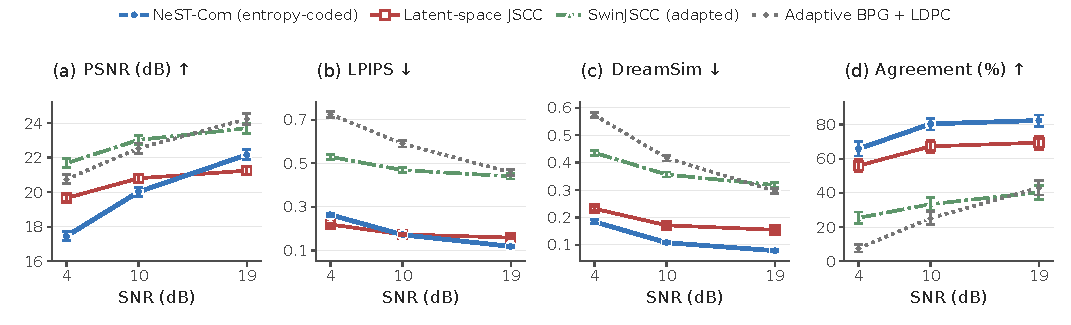
\includegraphics[width=\textwidth]{main_common500.pdf}
\caption{Reconstruction performance on common500 at $N=1024$. Markers are source-averaged means; bars are existing pointwise 95\% source-level intervals after averaging three noise draws. The entropy-coded 19-dB result is T1-C m10-corrected; latent-space JSCC and adapted SwinJSCC use their final 100k and 200k checkpoints. Agreement is the fraction whose ConvNeXt top-1 prediction matches that of the source image.}
\label{fig:main}
\end{figure*}

\subsection{Main Common500 Comparison}
Figure~\ref{fig:main} shows the full primary population. \ec{} achieves PSNRs of 17.448, 20.014 and 22.164 dB at 4, 10 and 19 dB, respectively. Its DreamSim decreases from 0.1839 to 0.0785 and agreement rises from 65.8\% to 82.4\%. At 4 dB, latent-space JSCC has higher PSNR (19.658 dB) and lower LPIPS (0.2188 versus 0.2633), while NeST-Com has lower DreamSim (0.1839 versus 0.2317) and higher agreement (65.8\% versus 55.9\%). The low-SNR result therefore expresses a fidelity/perceptual tradeoff, not dominance on every metric.

At 10 dB, LPIPS means are close (0.1715 versus 0.1733); the previously saved paired interval for their difference crosses zero. At 19 dB, NeST-Com's PSNR exceeds the latent-space baseline's 21.245 dB, while SwinJSCC and adaptive BPG retain higher PSNRs of 23.698 and 24.230 dB. NeST-Com has lower LPIPS and DreamSim than those two systems at all three displayed operating points. This is consistent with their different training losses and source priors; learned-feature preferences are not evidence that every generated detail is correct.

\subsection{Same-Prior Whole/Partial Comparison}
\begin{figure}[t]
\centering
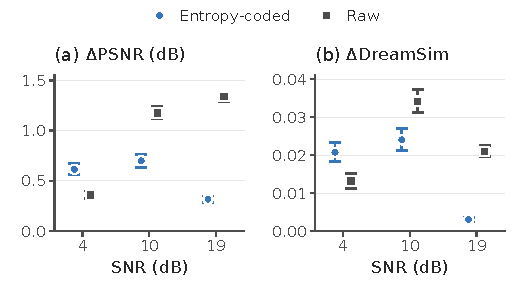
\includegraphics[width=\columnwidth]{paired_common500.pdf}
\caption{Within-family effects on common500. $\Delta$PSNR is partial minus whole; $\Delta$DreamSim is whole minus partial, so positive values indicate improvement. Bars are saved direct source-paired 95\% intervals. Entropy-coded results use the completed same-version audit and repair, including the corrected 19-dB endpoints. Raw retains its historical receiver rule.}
\label{fig:paired}
\end{figure}
The controlled internal comparison shares the prior and source-coding implementation while retaining the frozen family policies and expanding legal endpoints. After the version-consistency repair, the common500 PSNR gains at 4, 10 and 19 dB are 0.616 [0.564, 0.673], 0.701 [0.637, 0.766] and 0.319 [0.290, 0.349] dB. The corresponding DreamSim reductions are 0.02073, 0.02405 and 0.00304, with all three direct paired intervals excluding zero (Fig.~\ref{fig:paired}). These results connect the higher source utilization in Table~\ref{tab:utilization} to useful operating points of the frozen endpoint/MCS policies. They do not imply that every added endpoint helps every image or that the extra payload alone isolates every cause of the gain.

At corrected 19 dB, partial coding also improves LPIPS by 0.00520, DISTS by 0.00316 and MS-SSIM by 0.01014. Prediction agreement improves by 5.4 [2.0, 8.8] and 6.4 [3.8, 9.2] percentage points at 4 and 10 dB, but changes by $-0.2$ [$-2.0$, 1.6] at 19 dB. The latter does not support an agreement gain. The independent new100 comparison yields a 0.330 [0.269, 0.394] dB PSNR gain and identical agreement; this set is not pooled with common500 and retains its original four metrics.

\subsection{External Matched100 Comparison}
\begin{table*}[t]
\centering
\caption{Separate matched100 comparison at $N=1024$. Each cell is NeST-Com / ARPC adapted. All seven metrics and all 300 logical frames per method/SNR are included. Full-precision means, marginal intervals and direct paired intervals are supplied in the accompanying CSVs.}
\label{tab:arpc1024}
\small\setlength{\tabcolsep}{8pt}
\begin{tabular}{lrrr}
\toprule
Metric & 4 dB: NeST / ARPC & 10 dB: NeST / ARPC & 19 dB: NeST / ARPC \\
\midrule
PSNR (dB) $\uparrow$ & 17.064 / 13.656 & 19.612 / 16.127 & 21.742 / 17.819 \\
LPIPS $\downarrow$ & 0.2680 / 0.5193 & 0.1752 / 0.3507 & 0.1223 / 0.2567 \\
DISTS $\downarrow$ & 0.1949 / 0.3460 & 0.1528 / 0.2339 & 0.1260 / 0.1847 \\
DreamSim $\downarrow$ & 0.1845 / 0.5033 & 0.1077 / 0.3165 & 0.0796 / 0.2016 \\
DINO-L $\uparrow$ & 0.5502 / 0.1759 & 0.7227 / 0.3107 & 0.8105 / 0.5092 \\
Agreement (\%) $\uparrow$ & 64.0 / 21.0 & 79.0 / 45.0 & 85.0 / 74.0 \\
MS-SSIM $\uparrow$ & 0.5452 / 0.3028 & 0.7038 / 0.4672 & 0.8044 / 0.6114 \\
\bottomrule
\end{tabular}
\end{table*}

\arpc{} uses its official frozen adapted weights, paid compressed caption, native modes and boundaries, and independent receiver-side text encoding and source decoding. Caption length, source termination and alignment enter the charged source object. Both systems transmit under $68+956=1024$ symbols, the same nominal energy and their frozen finite-calibration policies. This aligns the link budget and source population, not the pretrained models' capacity, training corpus or compute.

ARPC's selected MCSs are QPSK $2/3$, 16-QAM $2/3$ and 64-QAM $5/6$. At 4 dB its actual endpoints are e3/e4; at 10 dB all are e5; at 19 dB they are e5/e6. All 900 ARPC logical frames parse successfully, with no post-output audit mismatch. The matched-source NeST-Com--ARPC PSNR differences are 3.408 [3.108, 3.728], 3.485 [3.263, 3.714] and 3.923 [3.700, 4.161] dB. Table~\ref{tab:arpc1024} reports all seven metrics and their directions.

These system-level differences include source representation, model, decoder, native syntax, endpoint availability and finite policy choices. They cannot all be attributed to within-scale truncation. In particular, native ARPC e7 requires a mean 8795 bits on these 100 sources, beyond the 4751-bit N1024 body capacity. The next section tests a larger budget that can carry both full representations.

\section{Budget Boundary at 2048 Channel Uses}
\subsection{Equal-Protection Two-Fragment Layout}
Each object uses two existing 1024-use subframes with equal protection. Both fragments pay 68 header symbols and 956 body symbols, a 13-bit length, CRC16 and a 96-bit reassembly record containing an object-CRC32 copy. At 64-QAM $5/6$, the two $k=4780$ information blocks leave 9296 source bits after fields and whole-byte alignment. No header, second length, CRC or reassembly cost is free. NeST source termination and its final byte padding remain included.

The two methods share the same 100 sources, SNRs and registered 2048-dimensional noise vectors, split into nonoverlapping contiguous fragment slices. Nominal total symbol energy is 4096. Both fragments and their reassembly checks must succeed; otherwise the entire output is gray. This experiment has no unequal protection, damaged-stream KEEP or truth-assisted repair.

\subsection{Fixed Complete-Representation Reference}
\begin{table*}[t]
\centering
\caption{Fixed complete-representation reference at $N=2048$, 19 dB, on the same 100 sources. Both methods correctly deliver 300/300 objects. Differences are NeST minus ARPC; intervals are direct source-paired 95\% intervals. Negative differences favor NeST for downward metrics.}
\label{tab:fixed2048}
\small\setlength{\tabcolsep}{9pt}
\begin{tabular}{lrrr}
\toprule
Metric & NeST full m10 & ARPC full e7 & Difference [95\% CI] \\
\midrule
PSNR (dB) $\uparrow$ & 22.913 & 21.107 & 1.806 [1.742, 1.871] \\
LPIPS $\downarrow$ & 0.1010 & 0.1376 & -0.0366 [-0.0395, -0.0340] \\
DISTS $\downarrow$ & 0.1152 & 0.1098 & 0.0054 [0.0024, 0.0086] \\
DreamSim $\downarrow$ & 0.0698 & 0.0783 & -0.0086 [-0.0119, -0.0052] \\
DINO-L $\uparrow$ & 0.8405 & 0.8228 & 0.0178 [-0.0018, 0.0386] \\
Agreement (\%) $\uparrow$ & 83.0 & 89.0 & -6.0 [-14.0, 2.0] \\
MS-SSIM $\uparrow$ & 0.8578 & 0.8235 & 0.0343 [0.0317, 0.0371] \\
\bottomrule
\end{tabular}
\end{table*}

The fixed reference sends complete NeST m10 and ARPC e7 using 64-QAM $5/6$ at all three SNRs. Both fit, but both deliver 0/300 objects at 4 dB and 0/300 at 10 dB. At 19 dB, both correctly deliver 300/300. Its low-SNR failure is a property of this fixed high-rate choice, not a claim that a larger budget inherently reduces reliability.

With complete reception at 19 dB (Table~\ref{tab:fixed2048}), NeST-Com improves PSNR by 1.806 [1.742, 1.871] dB, LPIPS by 0.03658, DreamSim by 0.00857 and MS-SSIM by 0.03429. ARPC has better DISTS: NeST minus ARPC is 0.00542 [0.00240, 0.00859]. The DINO difference of 0.01776 has interval [$-0.00180$, 0.03858]; agreement differs by $-6$ points with interval [$-14$, 2]. These intervals cross zero and do not prove equivalence. Comparing this full-representation reference with N1024 demonstrates a budget-dependent system tradeoff without assigning all remaining differences to transmitted-token count.

\subsection{Finite Low-SNR Adaptation}
The adaptive extension retains the equal-protection two-fragment protocol and both native complete-object syntaxes, with actual per-source fallback. Calibration evaluated exactly nine policy/SNR cells: NeST QPSK $1/2,2/3$ at 4 dB; NeST QPSK $2/3,3/4,5/6$ and 16-QAM $1/2,2/3$ at 10 dB; and ARPC QPSK $2/3$ at 4 dB and 16-QAM $2/3$ at 10 dB. Targets are the full legal endpoint of each method, not a guarantee that every source sends it. All original 1000 calibration sources and seeds 4101/4102/4103 were used. The explicit prospective nine-cell revision retained the earlier eight-cell scope as history; it allowed 27000 logical objects, 54000 subframes and 108000 header/body decoder attempts.

\begin{table}[t]
\centering
\caption{Frozen low-SNR $N=2048$ policies. DINO-L is the actual calibration mean over 1000 source averages, each containing three noise draws. These are calibration values, not test performance. ARPC denotes ARPC + LDPC--QAM (adapted).}
\label{tab:adaptivepolicies}
\footnotesize\setlength{\tabcolsep}{3.5pt}
\begin{tabular}{lcrr}
\toprule
Method & SNR (dB) & MCS & DINO-L \\
\midrule
NeST-Com & 4 & QPSK $2/3$ & 0.7208 \\
NeST-Com & 10 & 16-QAM $2/3$ & 0.8282 \\
ARPC (adapted) & 4 & QPSK $2/3$ & 0.2930 \\
ARPC (adapted) & 10 & 16-QAM $2/3$ & 0.5604 \\
\bottomrule
\end{tabular}
\end{table}

The completed calibration froze one policy per method/SNR using actual DINO-L after averaging the three noises within each source. Both methods selected QPSK $2/3$ at 4 dB and 16-QAM $2/3$ at 10 dB (Table~\ref{tab:adaptivepolicies}). NeST's selected calibration means are 0.720805 and 0.828199; ARPC's are 0.292956 and 0.560372. Exact ties follow the registered order: lower modulation order, lower nominal code rate, higher target, then lexical policy identifier. No tie or calibration interval triggered additional candidates, and calibration used no bootstrap. The search sets are asymmetric: NeST has two candidates at 4 dB and five at 10 dB, whereas ARPC has one at each. Equal final MCSs therefore do not imply equal search opportunity. These are choices within the nine specified cells, not evidence of a global optimum or estimates of test performance.

The completed frozen-policy test used external\_common100\_v1 at 4/10 dB with seeds 6201/6202/6203: 1200 objects, 2400 subframes and 4800 header/body decoder attempts. Each method/SNR cell correctly delivered all 300 objects; there were no null profiles, rejections or post-output payload mismatches. Thus the adaptive choices restored successful reception in this sample, whereas the separate fixed 64-QAM $5/6$ complete-object reference rejected all objects at these two SNRs. This change also permits actual per-source fallback, so it is not an isolated channel-code ablation or a claim that all received representations are complete m10/e7. With net source capacities of 2288/4848 bits at 4/10 dB, mean source occupancy is 94.90/94.76\% for NeST and 80.34/95.12\% for ARPC; only one of the 100 NeST sources uses m10 at 10 dB, while ARPC uses e4/e5 at 4 dB and e6 at 10 dB.

\begin{table*}[t]
\centering
\caption{Frozen-policy adaptive test at $N=2048$ on external\_common100. Each mean first averages three noises per source. $\Delta$ is NeST minus ARPC; brackets are the saved direct source-paired 95\% intervals. Negative differences favor NeST for downward metrics. Agreement differences are percentage points. The fixed-full 19-dB reference is separate.}
\label{tab:adaptive2048}
\footnotesize\setlength{\tabcolsep}{3pt}
\begin{tabular}{lrrrrrr}
\toprule
 & \multicolumn{3}{c}{4 dB} & \multicolumn{3}{c}{10 dB} \\
\cmidrule(lr){2-4}\cmidrule(lr){5-7}
Metric & NeST & ARPC & $\Delta$ [95\% CI] & NeST & ARPC & $\Delta$ [95\% CI] \\
\midrule
PSNR (dB) $\uparrow$ & 19.256 & 15.477 & 3.779 [3.493, 4.082] & 21.803 & 17.925 & 3.877 [3.688, 4.079] \\
LPIPS $\downarrow$ & 0.1879 & 0.4023 & -0.2144 [-0.2307, -0.1986] & 0.1212 & 0.2517 & -0.1306 [-0.1363, -0.1250] \\
DISTS $\downarrow$ & 0.1585 & 0.2713 & -0.1128 [-0.1246, -0.1013] & 0.1254 & 0.1822 & -0.0568 [-0.0612, -0.0521] \\
DreamSim $\downarrow$ & 0.1152 & 0.3810 & -0.2658 [-0.2933, -0.2386] & 0.0790 & 0.1965 & -0.1174 [-0.1309, -0.1049] \\
DINO-L $\uparrow$ & 0.7014 & 0.2715 & 0.4298 [0.3885, 0.4718] & 0.8129 & 0.5245 & 0.2884 [0.2474, 0.3304] \\
Agreement (\%) $\uparrow$ & 75.0 & 36.0 & 39.0 [28.0, 50.0] & 85.0 & 73.0 & 12.0 [2.0, 23.0] \\
MS-SSIM $\uparrow$ & 0.6822 & 0.4169 & 0.2653 [0.2456, 0.2854] & 0.8071 & 0.6176 & 0.1895 [0.1789, 0.2001] \\
\bottomrule
\end{tabular}
\end{table*}

Table~\ref{tab:adaptive2048} reports all seven test metrics. NeST-Com's PSNR is 19.256 versus ARPC's 15.477 dB at 4 dB and 21.803 versus 17.925 dB at 10 dB. The direct source-paired gains are 3.779 [3.493, 4.082] and 3.877 [3.688, 4.079] dB. DreamSim reductions are 0.26583 [0.23861, 0.29329] and 0.11740 [0.10491, 0.13090]; agreement gains are 39 [28, 50] and 12 [2, 23] percentage points. All fourteen pointwise paired intervals favor NeST-Com in the appropriate metric direction. They describe these two frozen adapted systems on the matched sources, not a multiplicity-adjusted guarantee or an endpoint-only causal effect.

The test first averaged the three noise draws within each source, then generated exactly one 10000-replicate source-paired bootstrap bank with seed 2026101902. Exact input/pixel/metric identities permitted reuse of 159 of the 400 distinct test image pairs; 241 pairs required new recovery and scoring (199 NeST and 42 ARPC). All 1200 logical frames remain in the denominator. Calibration and test together used the fixed 28200-object, 56400-subframe and 112800-decoder-attempt budget, with no further candidates. The 19-dB fixed-full reference remains separate: its complete-representation results include ARPC's lower DISTS and cross-zero DINO/agreement intervals. The low-SNR adaptive result therefore does not erase the high-SNR budget boundary or imply one calibrated policy across all three SNRs.


\subsection{Calibration Payload--Quality Diagnostics}
\begin{figure}[t]
\centering
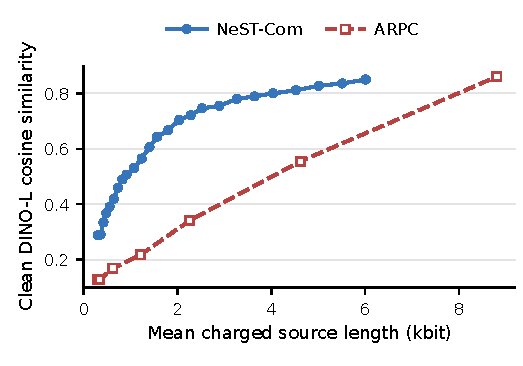
\includegraphics[width=\columnwidth]{cal100_payload_clean.pdf}
\caption{Cal100 clean source-coding diagnostic. Each marker is a native endpoint's saved mean charged source length and clean DINO-L over 100 sources. Straight segments join measured endpoint means. These are clean reconstructions, not wireless means; equal mean length does not imply equal per-image payload.}
\label{fig:capacity}
\end{figure}
The completed cal100 cache contains 2500 NeST and 700 ARPC clean source/endpoint states. Figure~\ref{fig:capacity} isolates their clean payload--quality relationship. At the same 2288-bit net source capacity, actual per-image fallback gives clean mean DINO 0.7166 for NeST and 0.3028 for ARPC; at 4848 bits it gives 0.8176 and 0.5546. These capacity-matched clean diagnostics help explain which representations are available before channel failures. They are not formal wireless quality means.

At the largest native endpoints, NeST m10 has mean charged length 6013 bits and clean DINO 0.8503; ARPC e7 has 8807 bits and 0.8607. Thus ARPC's clean top endpoint is not uniformly worse: it is slightly higher on this calibration metric at a larger source length. Mean-length points are not an exactly equal-rate per-image experiment and are not interpolated into unmeasured operating points.

\section{Auxiliary Evidence, Cost and Limitations}
\subsection{Actual Reconstructions and Raw Evidence}
\begin{figure*}[t]
\centering
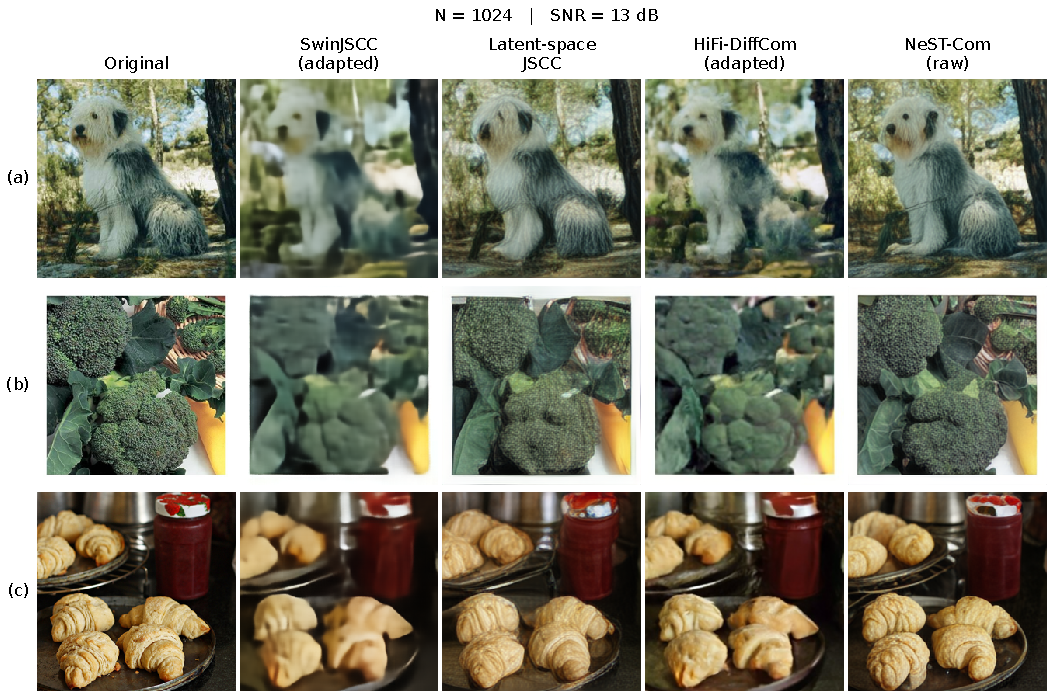
\includegraphics[width=0.9\textwidth]{fixed16_examples.pdf}
\caption{Previously selected fixed16 development examples at $N=1024$, 13 dB. These display examples were selected after viewing; all 16 images and their original pixels remain available. Latent-space JSCC uses 100k, SwinJSCC and HiFi's operators use 200k. Swin/HiFi share the same actual waveform and decoded auxiliary data. The NeST column is the historical raw implementation. The panel is illustrative, not a new quantitative sample or entropy-coded evidence.}
\label{fig:images}
\end{figure*}
Figure~\ref{fig:images} illustrates actual reconstruction behavior: transmitted coarse information constrains layout, while generated detail can remain incorrect. No sharpening, denoising or generative enlargement was applied. HiFi uses the original full 253-step posterior schedule and registered seed. On \emph{all} fixed16 images, its supplemental DISTS/DreamSim/MS-SSIM means are 0.24584/0.21807/0.82128; paired Swin's are 0.31659/0.35471/0.83837 and latent JSCC's are 0.19411/0.19116/0.75507. This descriptive development table does not become a common500 estimate or a confidence interval for a larger population.

Historical raw mismatch experiments and Kodak evidence retain their original variant and scope. The raw SNR-overestimation diagnostic showed large degradation; it motivates caution about accurate operating-point knowledge but is not an entropy-coded robustness test. The earlier two-group raw experiment's NO\_GO conclusion remains unchanged. No result from those studies is relabeled to support the present entropy-coded main claim.

\subsection{Versioned Shared-H800 Cost}
\begin{table}[t]
\centering
\caption{Existing shared-H800 mean latency (ms), $N=1024$, 19 dB, fixed16, batch one. Entropy rows are the old, pre-m10 version. Three fresh measured repetitions per source give 48 measurements per row; 4/10-dB rows and all components remain in the accompanying CSV.}
\label{tab:timing}
\footnotesize\setlength{\tabcolsep}{4pt}
\begin{tabular}{lrrr}
\toprule
Method & TX & RX & E2E \\
\midrule
Whole-scale (raw) & 136.3 & 571.6 & 708.0 \\
NeST-Com (raw) & 105.8 & 349.5 & 455.3 \\
Whole-scale (entropy) & 243.0 & 468.7 & 711.8 \\
NeST-Com (entropy) & 938.3 & 504.0 & 1442.3 \\
Latent-space JSCC & 15.6 & 22.6 & 38.3 \\
SwinJSCC (adapted) & 28.1 & 21.9 & 50.1 \\
\bottomrule
\end{tabular}
\end{table}

Table~\ref{tab:timing} reuses completed shared-H800 measurements, with batch one, the fixed16 development sources and three fresh measured repetitions following three fresh warmups at each condition. All 1728 calls completed, including 864 measurements. TX includes fresh source encoding and actual fallback attempts; RX includes real receive processing and reconstruction. Software end-to-end latency excludes separately recorded channel-noise generation and pure provenance-audit overhead. All receiver outcomes remain in the measurements.

The grid combines 576 unchanged successful calls from the stopped v5 attempt and 1152 from the v6 recovery. One failed initial entropy warmup is archived and contributes an extra known visual-encoder attempt, not a completed measurement. The shared device/software match, but resident workloads and admission conditions differ between segments; these are not uncontended latencies. The entropy rows predate the m10 revision and are not asserted to be revised m10 delays. ARPC's stage wall times on another machine include initialization and I/O and are not converted into cross-hardware speedup ratios. Raw avoids TX autoregressive inference, but its different source/failure interface and measured quality must accompany any complexity comparison.

\subsection{Interpretation Limits}
The channel is AWGN with the registered energy convention. There is no fading, feedback, retransmission or learned power control. Candidate sets and calibration budgets are finite; a selected policy is not globally optimal. Reuse requires actual source/event/pixel and scoring identity, not merely a matching endpoint. All failures are retained, and unknown execution failures are recorded independently of legitimate link rejection.

The internal same-prior comparisons support the value of a finer legal transmission interface. The low-SNR N2048 test shows that a larger frame still needs an appropriate MCS and actual source fallback: the fixed high-rate reference fails where the finite adaptive policies succeed. Its uniformly favorable pointwise test intervals do not remove the fixed-full 19-dB metric conflicts. The external results compare complete adapted systems. Pretraining scale, native text conditioning, decoder adaptation, numerical environments and method-specific source procedures are not controlled into a common backbone. Different quality metrics answer different questions, and generated plausibility does not establish source fidelity. The matched100 subset, independent new100, common500 and fixed16 development results remain separate.

\section{Conclusion}
NeST-Com turns legal within-scale token endpoints into a fully charged digital interface. Actual terminated lengths drive a frozen fallback chain, a paid profile specifies the endpoint and layout, and an isolated receiver recovers transmitted tokens before generating unsent representation. The corrected N1024 same-prior comparison supports gains from finer endpoints while retaining low-SNR fidelity limitations. In the N2048 matched-source test, finite low-SNR adaptation restores reception and favors NeST-Com on all seven measured metrics at 4/10 dB. The separate complete-representation test at 19 dB retains ARPC's DISTS advantage and cross-zero DINO/agreement intervals. Budget, link policy and native representation jointly determine the observed system tradeoff; neither a universal metric advantage nor an endpoint-only explanation follows.

\appendices
\section{Reproducibility and Evidence Boundaries}
The accompanying source manifest maps each table and figure to immutable result files and their SHA256 digests. Primary N1024 partial-family quality uses the frozen 4/10-dB results and corrected T1-C 19-dB results; its same-prior comparison uses the completed whole-family version repair. New100 is never merged into common500. The paid-stream utilization audit is separately traceable. The external100 N1024 comparison, fixed-full N2048 reference and low-SNR adaptive N2048 evaluation each preserve their original registrations, actual waits, full logical denominators and source-paired statistics. The adaptive test used 241 new and 159 reused distinct image-pair scores while retaining all 1200 logical frames; its single source-bootstrap bank is preserved. Full CSVs retain precision beyond the rounded values printed here. Historical metadata, host-location and test-fixture failures are retained with their actual nonzero exits; they are not recast as successful scientific calls, and closed model outputs were not rerun to resolve them.

No training, baseline reconstruction, rescoring, bootstrap or timing is performed by the manuscript build. Figures reuse reviewed exports or deterministically draw saved means; table generation reads saved summaries. Author names, affiliations, funding, corresponding author and target-journal page constraints require author input and are listed in the delivery note; no identities are fabricated in this review copy.
